% Version 2018

\subsubsection{Instrumentos de vuelo}
\label{sec:instrumentos.de.vuelo}


\begin{frame}{Instrumentos de vuelo}

  \begin{block}{Definici\'on}
    Instrumentos que se utilizan para mostrar informaci\'on de la
    aeronave y controlar la orientaci\'on de la misma durante el vuelo
  \end{block}

  \begin{columns}{2}

    \begin{column}{0.5\textwidth}
{\small
  \begin{block}{    Necesidades a cumplir:}
    \begin{itemize}
    \item Permitir volar en condiciones de clim\'aticas desfavorables, 
	con escasa visibilidad y durante la noche
    \item Asegurar una operaci\'on segura y confiable
    \item Dar avisos tempranos sobre cualquier falla en los sistemas
      de la aeronave o partes de la misma, de forma que los pilotos
      puedan tomar una acci\'on inmediata
    \end{itemize}
  \end{block}
}
\end{column}
    \begin{column}{0.5\textwidth}
 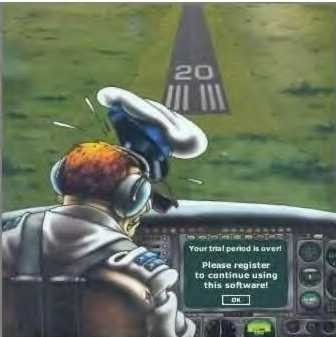
\includegraphics[width=\linewidth]{imagenes/1.1.introduccion/problema_soft.jpg} \\
    \end{column}
  \end{columns}

\end{frame}

\begin{frame}
  
  \begin{alertblock}{}
    La habilidad de capturar y transmitir toda la informaci\'on que un piloto requiere, de forma segura y f\'acil de entender, ha sido un desaf\'io a trav\'es de la historia de la aviaci\'on.\\
{\tiny Referencia:  \cite{FAA_hdk_aMThA_v2}}
  \end{alertblock}

        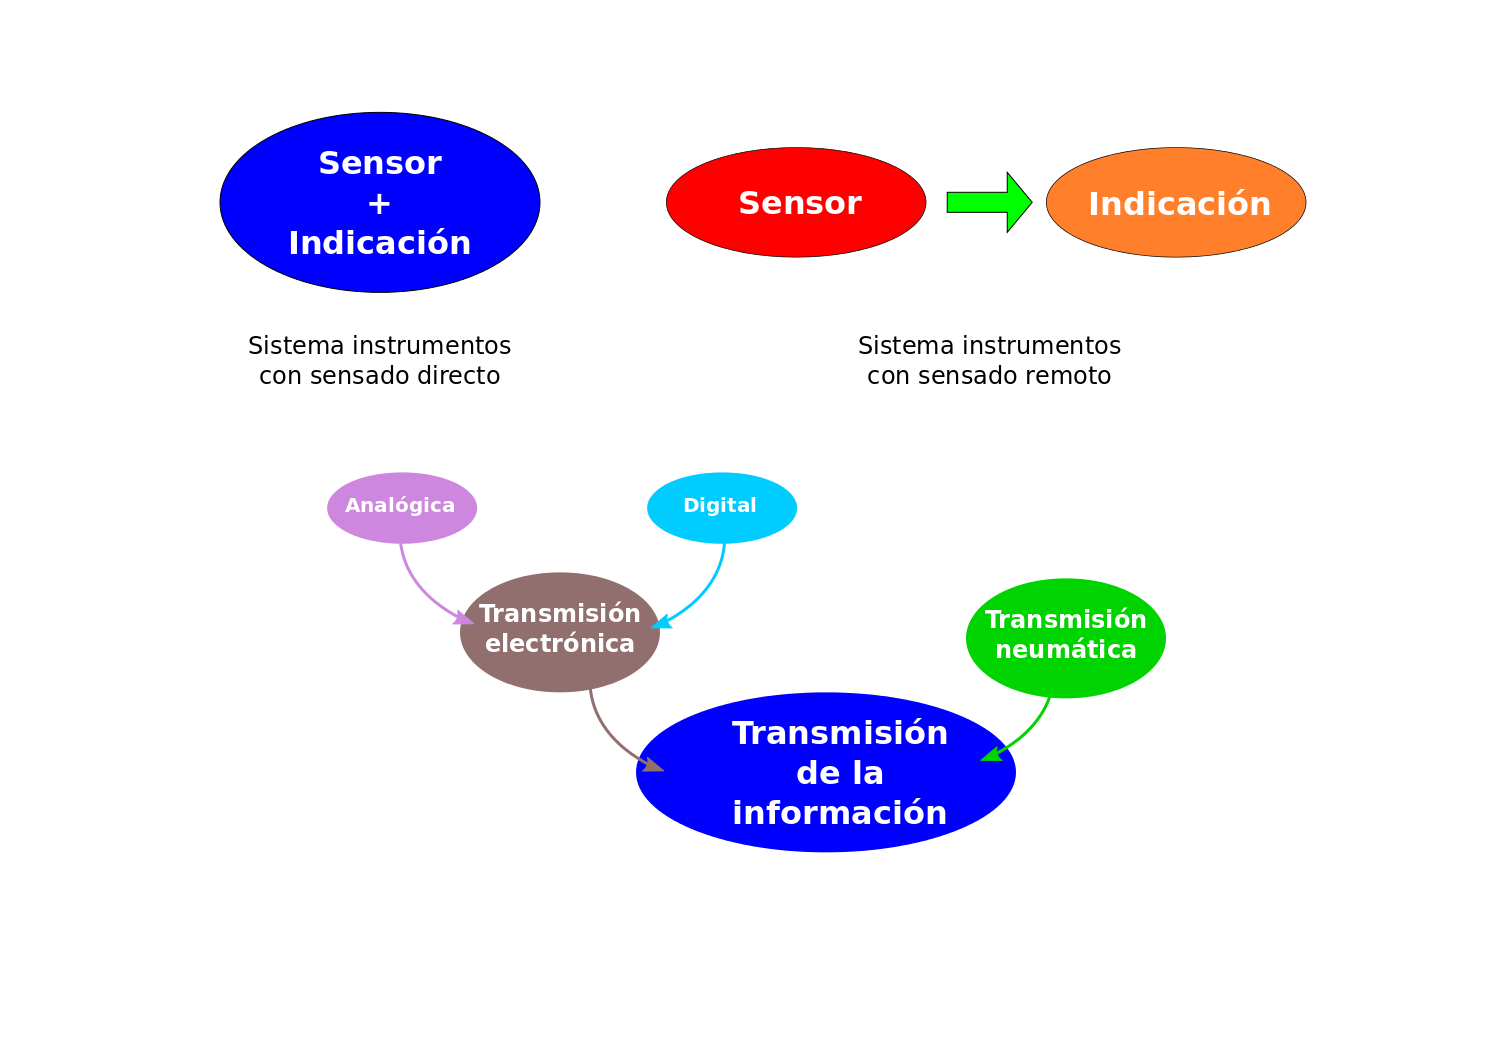
\includegraphics[width=\textwidth]{tikz/01_sistema_instrumentos.png}

        {\tiny Adaptado de: \cite{FAA_hdk_aMThA_v2}}





%   \begin{columns}
%     \begin{column}{0.5\textwidth}
%       \begin{block}{Sistema de instrumentos}
%         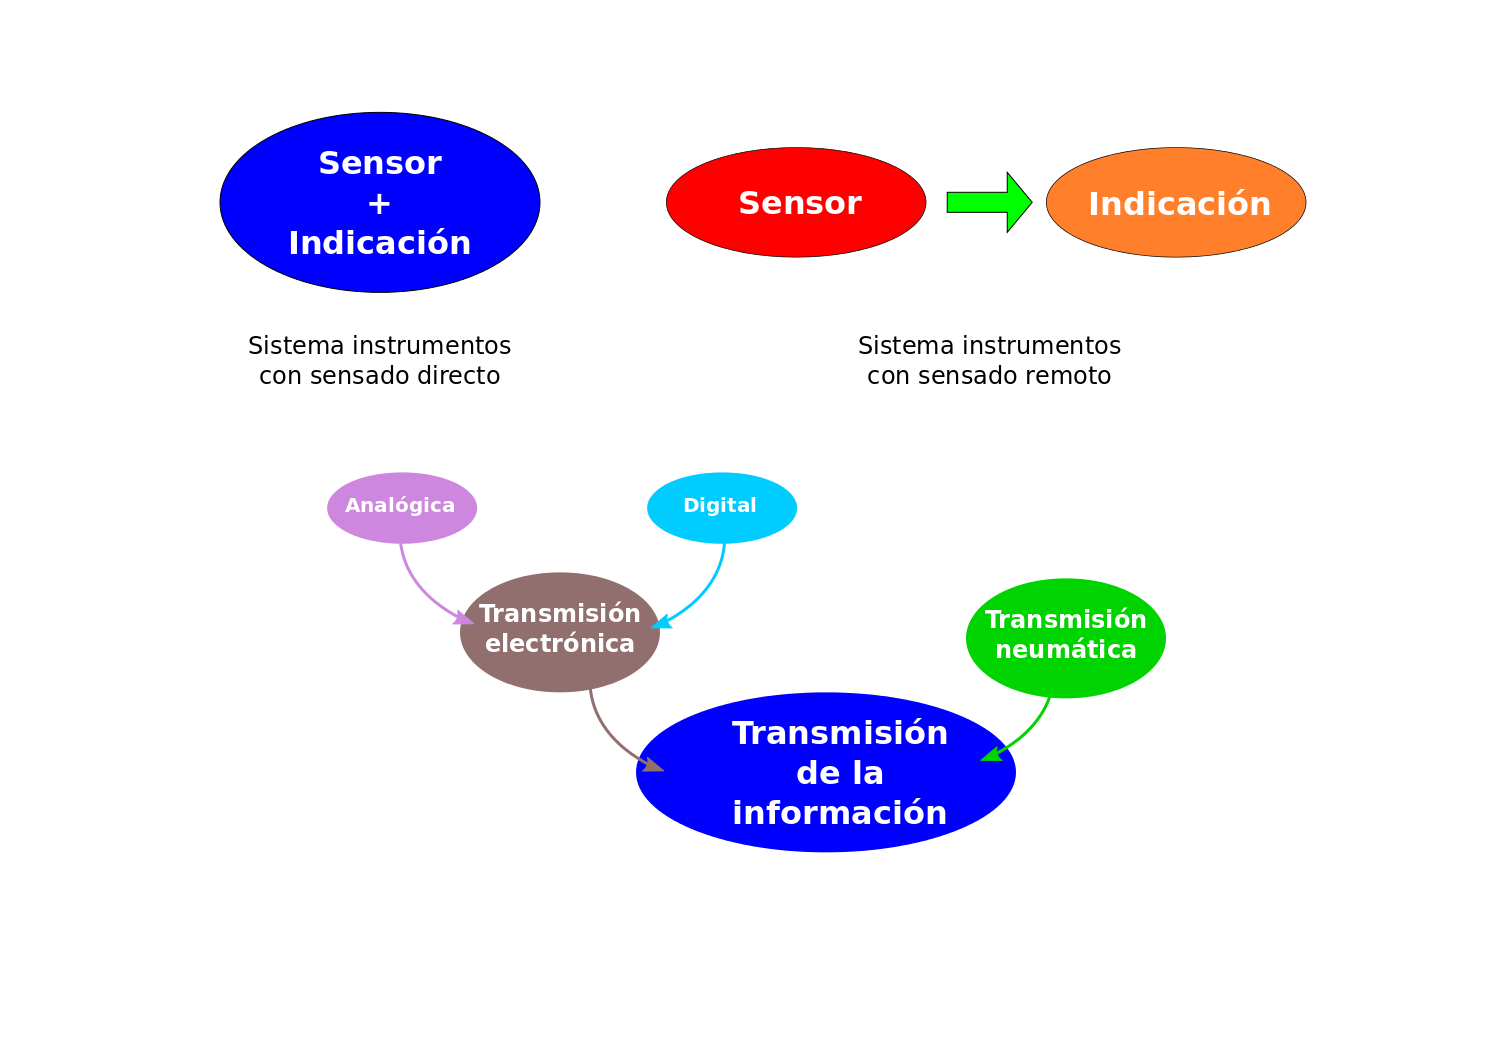
\includegraphics[width=\linewidth]{tikz/01_sistema_instrumentos.png}

%         {\tiny Adaptado de: \cite{FAA_hdk_aMThA_v2}}
%       \end{block}
%     \end{column}
%     \begin{column}{0.5\textwidth}
%   % \begin{minipage}[b]{0.5\textwidth}
%     \begin{block}{Transmisi\'on de la informaci\'on}
%       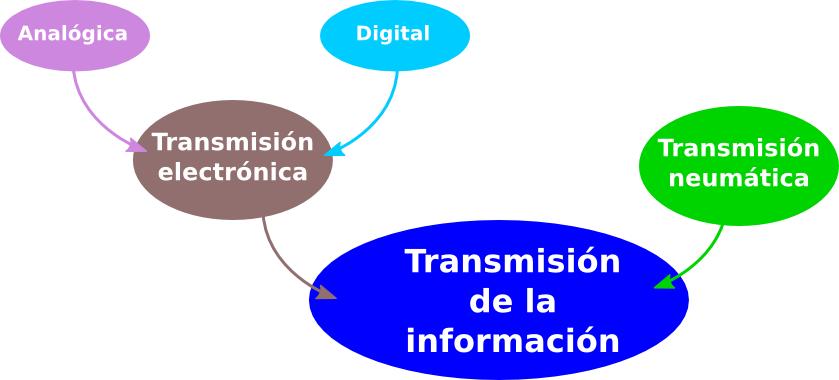
\includegraphics[width=\linewidth]{tikz/01_transmision_informacion.png}
%     \end{block}
%   % \end{minipage}
%   \end{column}
% \end{columns}

\end{frame}

\subsubsection{Ergonom\'ia}
\label{sec:ergonomia}

%	01.01.01.Ergonomia
%	version 2018


\begin{frame}

      \begin{block}{Ergonom\'ia}
        \emph{Del gr. 
	\griego{\'ergon}
''ergon'' (trabajo) y 
``nom\'ia'' ( \griego{n\'omos} ``nomos'' (regla, ley), 
	m\'as el sufijo ``ia'' (cualidad))}\\
1. f. Estudio de la adaptaci\'on de las m\'aquinas, muebles y utensilios a la persona que los emplea habitualmente, para lograr una mayor comodidad y eficacia.\\
2. f. Cualidad de ergon\'omico (adaptado a las condiciones del usuario). \emph{El puesto de conducci\'on tiene buena ergonom\'ia.}

{\tiny Fuente: Real Academia Espa\~nola }

\vspace{3mm}

\emph{La Ergonom\'ia (o Factores Humanos) es la disciplina cient\'ifica relacionada con la comprensi\'on de las interacciones entre los seres humanos y los elementos de un sistema, y la profesi\'on que aplica teor\'ia, principios, datos y m\'etodos de dise\~no para optimizar el bienestar humano y todo el desempe\~no del sistema.
}

{\tiny Fuente: Asociaci\'on Internacional de Ergonom\'iía (IEA) \,
\url{https://www.iea.cc/whats/}}
      \end{block}

\end{frame}

\begin{frame}{}
  \begin{block}{Ergonom\'ia Cognitiva}
    ``Se ocupa de los procesos mentales, tales como la percepci\'on, la memoria, el razonamiento y la respuesta motora, que afectan a las interacciones entre los seres humanos y otros elementos de un sistema. %Los temas relevantes incluyen carga de trabajo mental, la toma de decisiones, el rendimiento experto, la interacci\'on persona-computadora, la fiabilidad humana, el estr\'es laboral y la forma como estos pueden estar relacionados con el dise\~no de los sistemas humanos. La ergonom\'ia cognitiva estudia los procesos de cognición en el trabajo y ajustes operativos, a fin de optimizar el bienestar humano y el rendimiento del sistema
"

{\tiny Fuente: Asociaci\'on Internacional de Ergonom\'iía (IEA) \,
\url{https://www.iea.cc/whats/}}

  \end{block}

\vspace{3mm}

El campo de la ergonom\'ia cognitiva surgi\'o predominantemente en los a\~nos 70 con la llegada de la computadora personal y los nuevos desarrollos en los campos de la psicolog\'ia cognitiva y la inteligencia artificial. Se contrasta con la tradici\'on de la ergonom\'ia f\'isica porque ``\emph{la ergonom\'ia cognitiva es... la aplicaci\'on de la psicolog\'ia al trabajo... para lograr la optimizaci\'on entre la gente y su trabajo.}''

{\tiny Fuente: \url{https://es.wikipedia.org/wiki/Ergonom\%C3\%ADa_cognitiva}}

\vspace{3mm}

Mayores detalles pueden consultarse en \cite{van_der_Veer} \\
{\tiny \url{https://pdfs.semanticscholar.org/ea75/ca4d902bc5089c8542751e7ed03c97c13197.pdf}
}


\end{frame}

   
\begin{frame}{Modelo de procesamiento de informaci\'on humano}

  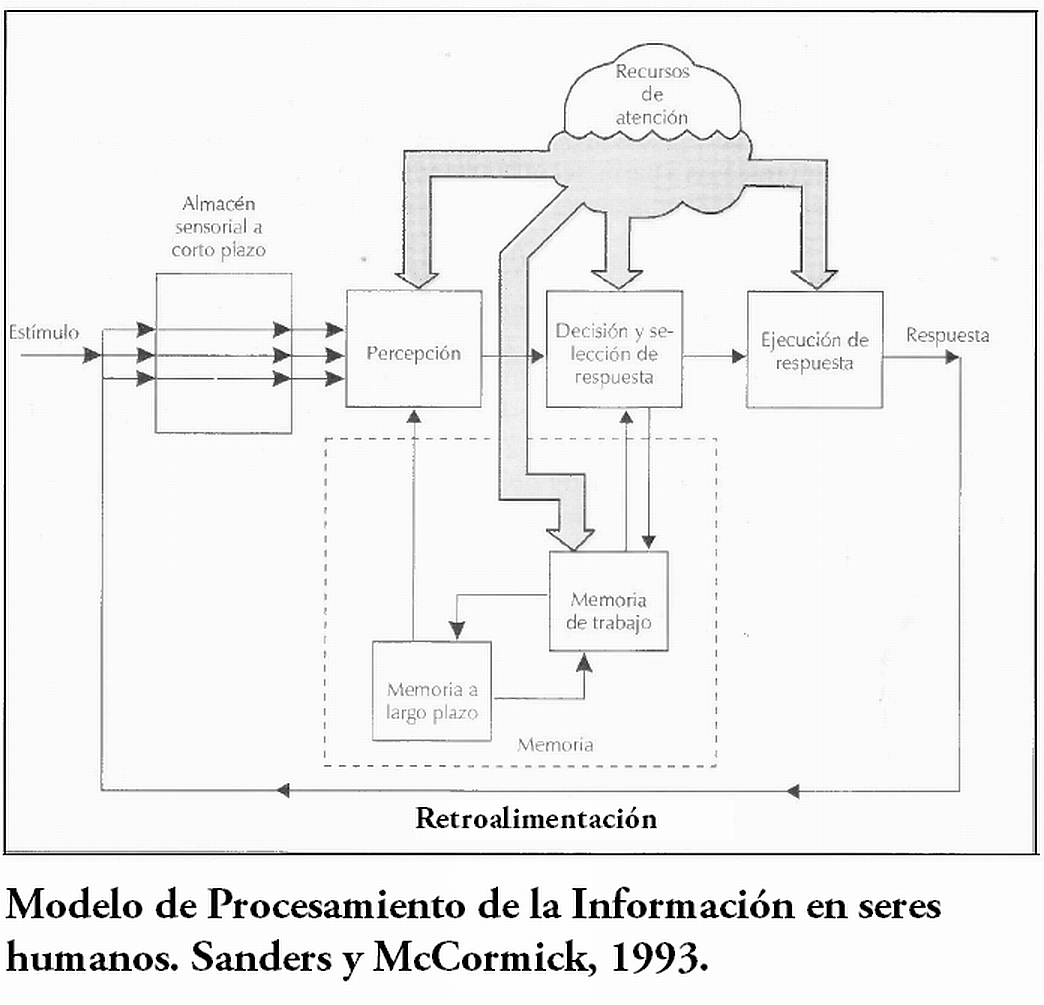
\includegraphics[width=0.6\linewidth]{imagenes/1.1.introduccion/modelo_procesamiento_informacion.png}

{\tiny Fuente: Romosquera, \url{https://commons.wikimedia.org/wiki/File:Procesamiento_de_la_Informaci\%C3\%B3n.png}
\\ \cite{mark1993human} }

\end{frame}

\begin{frame}{Ergonom\'ia F\'isica}
  
\end{frame}

\begin{frame}{Ergonom\'ia Visual}
  
\end{frame}



\begin{frame}

  \begin{columns}
    \begin{column}{0.45\textwidth}
      \begin{block}{Sistema de ciclo cerrado persona-m\'aquina}
        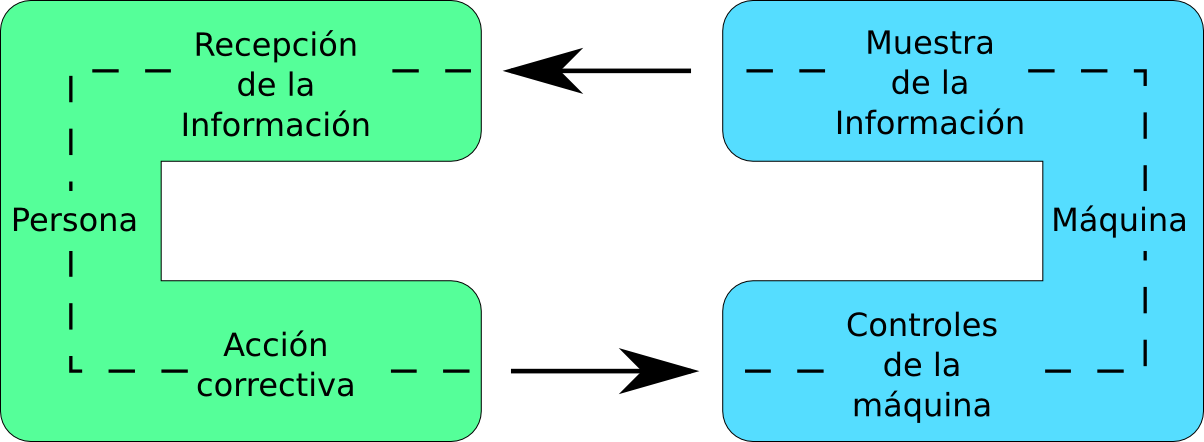
\includegraphics[width=\linewidth]{tikz/01-03-loop-persona-maquina.png}

        {\tiny Adaptado de \cite{bhandari2010design}}
      \end{block}
    \end{column}

    \begin{column}{0.05\textwidth}
    \end{column}

    \begin{column}{0.45\textwidth}

    \end{column}
      
  \end{columns}

\end{frame}



\subsubsection{Formas de presentaci\'on de la informaci\'on}
\label{sec:formas.presentacion.informacion}

%	01.01.01. Formas de presentaci\'on informaci\'on
%	version 2018



\begin{frame}{Formas de presentaci\'on de la informaci\'on}

  \begin{itemize}
  \item {\bf Presentaciones cuantitativas}
    \begin{itemize}
      \item Escala circular
      % \begin{itemize}
      %    \item Escala lineal
      %    \item Escala no lineal (cuadr\'atica, logar\'itmica}
      % \end{itemize}
       \item Escala longitudinal
    \end{itemize}
  \item {\bf Presentaciones cualitativas}
  \item {\bf Presentaciones directoras}
  \end{itemize}

\end{frame}

\begin{frame}{Presentaciones cuantitativas
	}

  \begin{tabular}{ccc}
    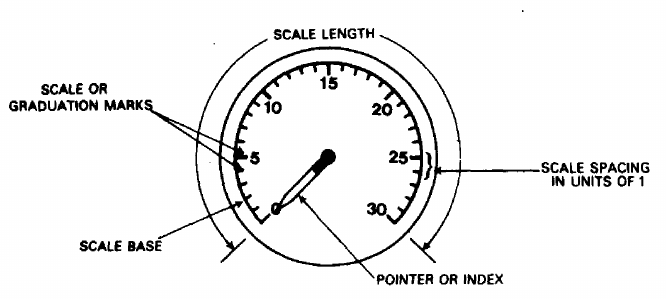
\includegraphics[width=0.45\textwidth]{imagenes/1.2.clasificacion.instrumentos/escala_circular_cuantitativa.png} & \hspace{3mm}
&     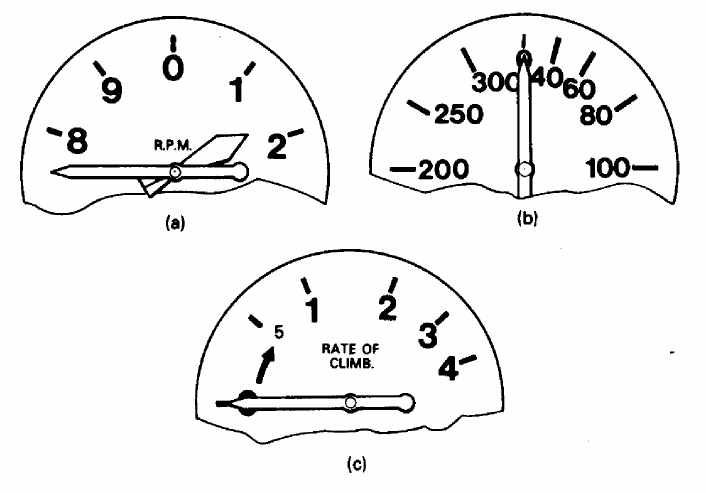
\includegraphics[width=0.45\textwidth]{imagenes/1.2.clasificacion.instrumentos/escala_circular_lineal_no_lineal.png}
\\
	Escala circular cuantitativa & 
& \parbox{0.45\textwidth}{a) Lineal, b) ley cuadr\'atica, \\c) ley logaritmica}
\\
  \end{tabular}

{\tiny Referencia: \cite{pallett1992aircraft}}

\end{frame}

\begin{frame}{Presentaciones cuantitativas
	}

  \begin{tabular}{ccc}
    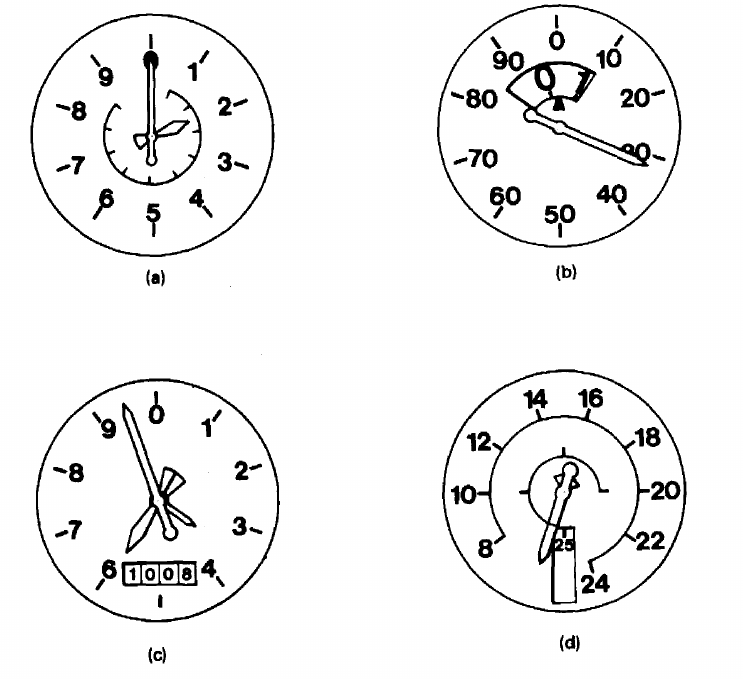
\includegraphics[width=0.45\textwidth]{imagenes/1.2.clasificacion.instrumentos/escala_gran_alcance.png} & \hspace{3mm}
&     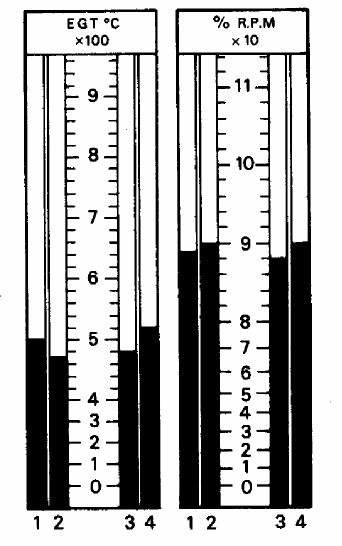
\includegraphics[width=0.35\textwidth]{imagenes/1.2.clasificacion.instrumentos/longitudinal.png}
\\
\parbox{0.45\textwidth}{\small a)Escalas conc\'entricas, (b) escalas fijas y giratorias, (c) escala com\'un tres agujas, (d) aguja dividida}
&
& {\small Escala longitudinal}
\\
  \end{tabular}
{\tiny Referencia: \cite{pallett1992aircraft}}
\end{frame}

\begin{frame}{Clasificaci\'on de los Instrumentos}

  \begin{tabular}{ccc}
    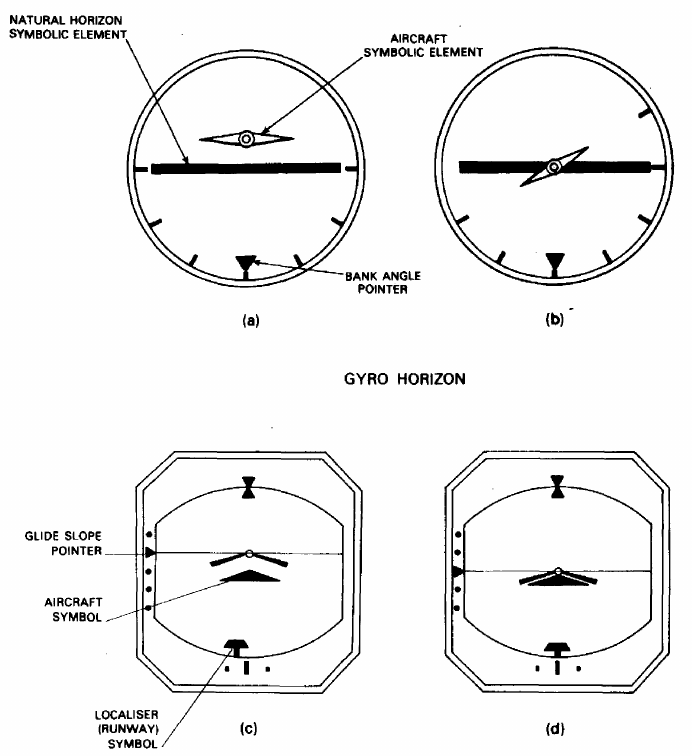
\includegraphics[width=0.45\textwidth]{imagenes/1.2.clasificacion.instrumentos/director.png} & \hspace{3mm}
&     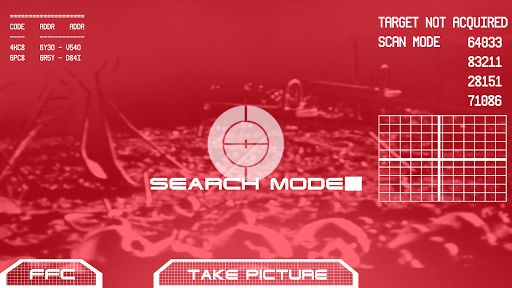
\includegraphics[width=0.5\textwidth]{imagenes/1.2.clasificacion.instrumentos/terminator_hud.png}
\\
\parbox{0.45\textwidth}{Director de vuelo}
&
& Terminator Hud
\\
  \end{tabular}

\end{frame}

\begin{frame}{Clasificaci\'on de los Instrumentos}

{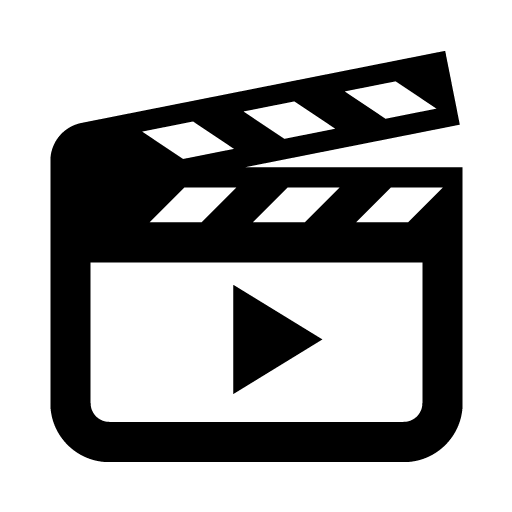
\includegraphics[width=0.1\textwidth]{imagenes/Video.png}}\,
The Evolution of the Head-Up Display \url{https://www.youtube.com/watch?v=ypIbmfm7n8A}
\vspace{3mm}

  \begin{tabular}{ccc}
    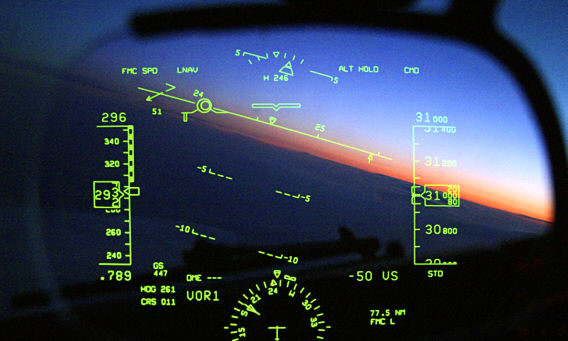
\includegraphics[width=0.45\textwidth]{imagenes/1.2.clasificacion.instrumentos/hud.jpg} & \hspace{3mm}
&     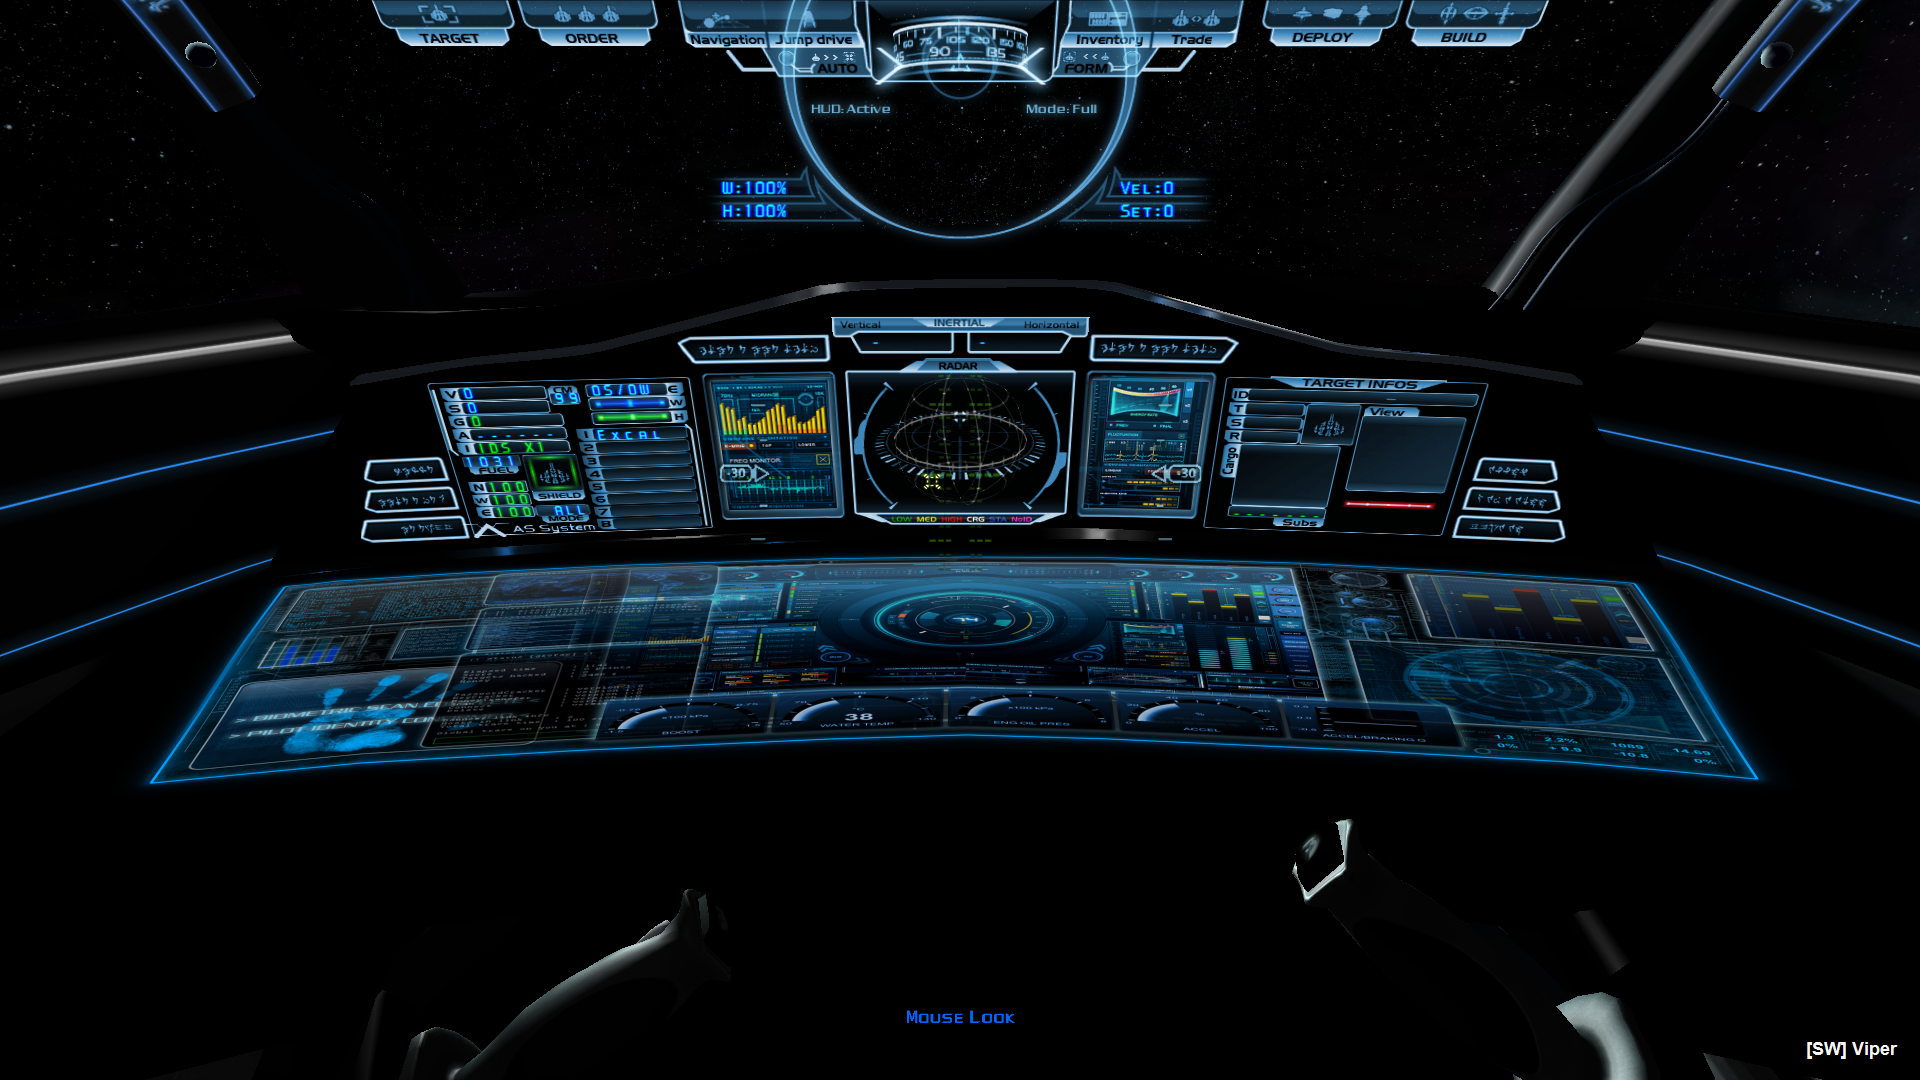
\includegraphics[width=0.5\textwidth]{imagenes/1.2.clasificacion.instrumentos/viper_11.png}
\\
\parbox{0.45\textwidth}{Head Up Display}
&
& Hud futuro
\\
  \end{tabular}

\end{frame}

\begin{frame}{Clasificaci\'on de los Instrumentos}



\vspace{3mm}

{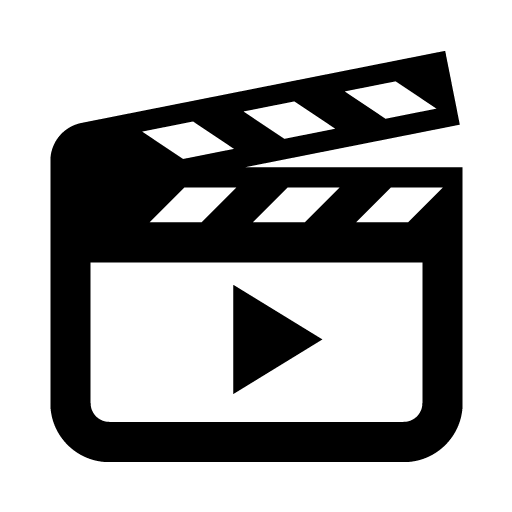
\includegraphics[width=0.1\textwidth]{imagenes/Video.png}}\,
Enhanced Flight Vision System \url{https://www.youtube.com/watch?v=DR9lyAM2YNE}

\vspace{3mm}

  \begin{tabular}{ccc}
    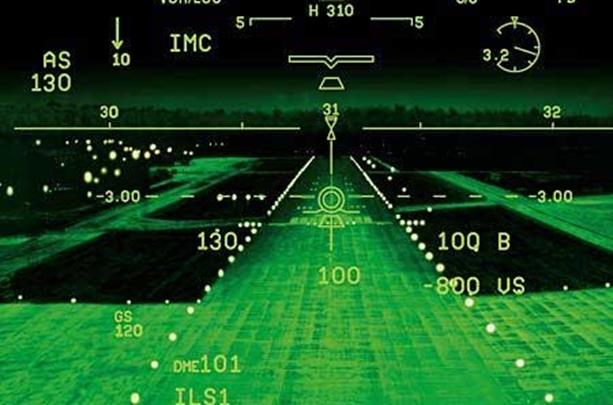
\includegraphics[width=0.45\textwidth]{imagenes/1.2.clasificacion.instrumentos/EFVS_Photo.jpg} & \hspace{3mm}
    &     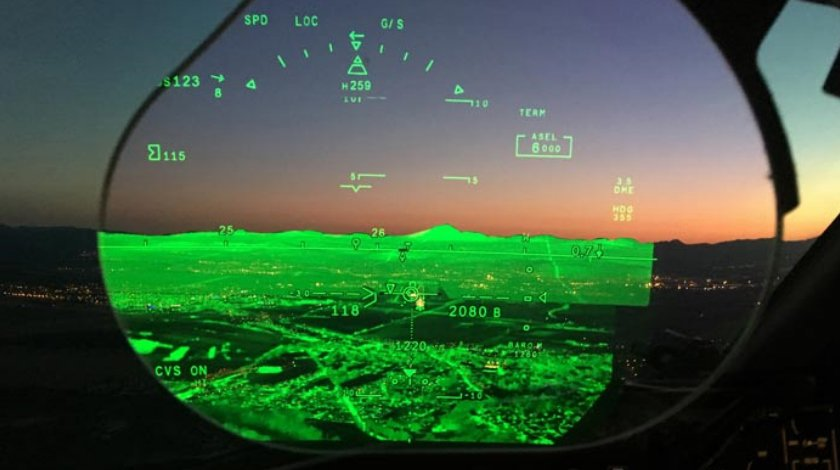
\includegraphics[width=0.45\textwidth]{imagenes/1.2.clasificacion.instrumentos/efvs.jpg} \\
  \end{tabular}
  

\end{frame}
